\documentclass[conference,letterpaper]{IEEEtran}
\usepackage[T1]{fontenc}
\usepackage{amsmath,amssymb,booktabs,graphicx}
\usepackage[hidelinks]{hyperref}
\newcommand{\BA}{\mathrm{BA}}
\title{[Experiment, Analysis, and Benchmark] Access-Conditioned Decision Decomposition for Auditing Cross-Dataset Motor-Imagery EEG Decoders}
\author{\IEEEauthorblockN{Author names and affiliations pending confirmation}}
\begin{document}
\maketitle
\begin{abstract}
A decision benchmark can report a gain when its fitted rule has seen trials that would be unavailable at prediction time. A positive cohort mean can also conceal how often a particular deployed model makes participants worse off. We study these problems in four discovery datasets (224 participants), locked confirmation (87), and an external repeated-session cohort (62). Access-conditioned decision decomposition (ACDD) records the information available to fit each rule, its evaluation trials, its label-informed diagnostic reference and the order of aggregation. On 62 Stieger2021 participants, fitting a threshold to ten unlabeled scores and scoring subsequent trials moved balanced accuracy from 53.04\% to 54.45\% for EEGNet and from 51.18\% to 52.93\% for a compact EEG-Conformer. Both gains fell below the prespecified two-point criterion. For each backbone, one participant lost more than two points after gains were averaged across 15 model configurations. At a fixed configuration, the counts ranged from 1 to 14 and from 0 to 17 of the same 62 participants. On the same protected trials, the two evaluated posterior-at-0.5 rules (EM and ridge BBSE) reduced mean BA. A common-suffix replay separates changes in the threshold-fitting budget from changes in the evaluation sample. The results delimit what a benchmark on previously generated EEG scores can establish about deployment.
\end{abstract}
\begin{IEEEkeywords}
benchmarking, data provenance, temporal evaluation, electroencephalography, cross-dataset validation
\end{IEEEkeywords}
\section{Introduction}\label{sec:intro}
Consider a benchmark operator who receives a chronologically ordered stream of target scores. A threshold fitted to the first ten scores can be evaluated on the whole stream or only on rows eleven onward. Both queries may appear under the same prefix-ten label in a results table. Only the latter measures performance on trials unseen by that fixed threshold. Another ambiguity arises after evaluation. Counting participants who lose accuracy after averaging over 15 models answers a different question from counting those who would lose accuracy if one particular model were deployed.

These ambiguities matter for motor-imagery EEG. Decoder performance varies with the acquisition, training population and participant~\cite{jayaram2018,eder2024}. In binary classification, an ordering measure such as AUC is invariant to a change of operating threshold~\cite{fawcett2006}. Balanced accuracy (BA), the mean of the two class recalls, depends on that threshold~\cite{brodersen2010}. A gain in BA can therefore occur without a change in the information carried by the representation. Conversely, even useful score ordering can yield poor absolute decisions.

We study these questions with access-conditioned decision decomposition (ACDD), an audit of frozen decoder outputs. The contributions are an empirical comparison of declared information and evaluation windows, a measurement of how model aggregation changes participant-degradation counts, and a trial-level replay with identifiable inputs. We retain the historical cohort endpoints, gate decisions and adverse controls. The experimental variation lies in what an evaluator can read and how it aggregates outcomes. Model architecture and training are fixed.
\section{Benchmark design and related work}\label{sec:benchmark}
\subsection{Which records define an experiment?}
TimeEval organizes time-series anomaly benchmarks through algorithm, dataset and parameter combinations, with separate execution and evaluation stages~\cite{timeeval}. In our setting, two runs with identical model, dataset and policy parameters can still define different comparisons. We record two further components for each result, the rows admitted to fitting and the rows admitted to evaluation. The experimental key also retains the checkpoint, source condition, seed, participant, session and trial order. Its output identifies the matched default decision, access-conditioned decision and any diagnostic that used labels. Our artifact maps these keys to hashed exports, individual outcomes and table rows.

The Dataflow model separates the event-time window to which an observation belongs from when a computation emits a result~\cite{dataflow}. Our narrower problem has a recorded order and a finite participant stream. For a decision on trial $j$, rows can belong to a participant's analysis window while being unavailable when the threshold is fitted. Separating these row sets exposes future access even if each policy eventually reports one number per person. Late-arriving messages, watermarks and processing throughput are outside this experiment.

Schmidl \emph{et al.} explain why a threshold-independent evaluation can give full credit when some threshold separates all cases~\cite{tschmidl}. Here the operating threshold itself is in question. We measure both ordering and the decision achievable with a declared fit window. A label-informed reference then measures how much a fitted rule leaves unexplained. Its availability during evaluation gives it no role in fitting a target policy.

\subsection{Cohorts and the freeze}
Discovery pools 224 participants across BNCI2014-001 (9), Cho2017 (52), PhysioNetMI (109) and Lee2019-MI (54)~\cite{tangermann2012,cho2017,schalk2009,lee2019}. Locked confirmation uses 87 Dreyer2023 participants~\cite{dreyer2023}. External evaluation uses 62 Stieger2021 participants with repeated sessions~\cite{stieger2021}. The historical prefix-ten endpoint scores the full record, including the first ten trials. The protected Stieger endpoint scores only subsequent trials.

The Stieger register crosses two backbones, five training conditions, three seeds (17, 29 and 43), and three preprocessing/normalization candidates. All 90 registered inference units completed. The prespecified candidate uses raw input and BatchNorm (raw-BN). Its 30 units use EEGNet~\cite{lawhern2018} or a compact EEG-Conformer~\cite{song2023}, with four single-source conditions and one multi-source leave-one-dataset-out condition per backbone. Each checkpoint was selected by mean participant BA on held-out source-validation participants. Those participants also contribute to source calibration. Their results cannot serve as independent source-test evidence. All target decision analyses retain the original checkpoints.
\subsection{Evidence phases and decision points}
Figure~\ref{fig:workflow} traces a frozen score from its cohort and model to the trials that may set the threshold and the trials on which its decisions are judged.
\begin{figure*}[t]
\centering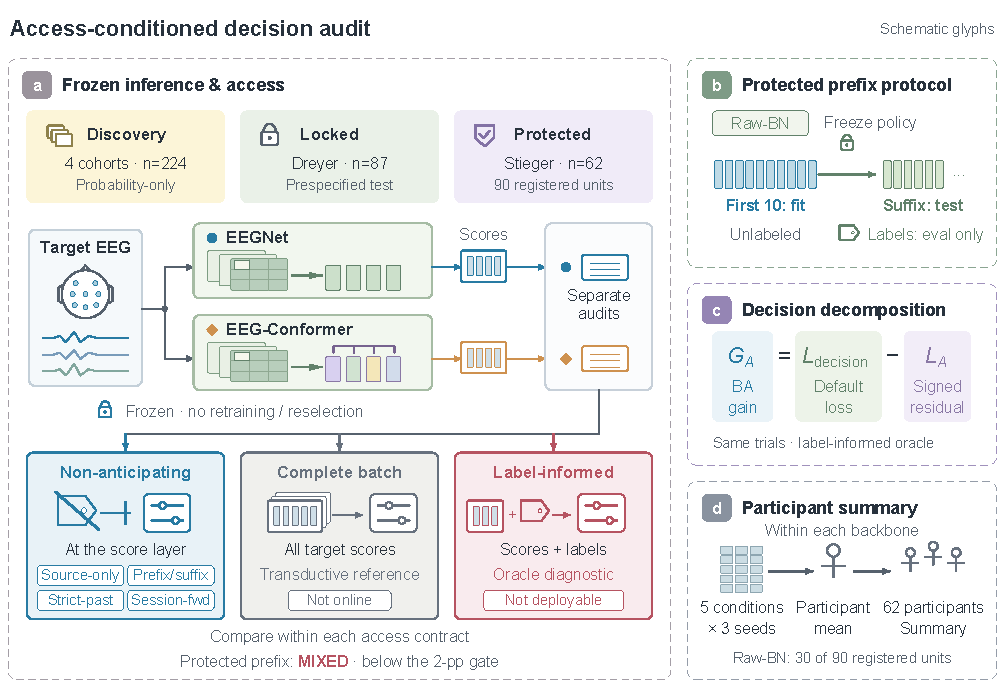
\includegraphics{figures/figure1_acdd_workflow.pdf}
\caption{Decision audit across three evidence phases. (a) Access is specified at the interface of already generated scores. Source-only, fixed-prefix, strict-past and session-forward rules exclude future target scores and target labels from threshold fitting. Complete batch reads future scores. The oracle uses evaluation labels. (b) The protected fit sees the first ten scores and is held fixed thereafter. (c) Each decomposition uses the same evaluation trials for policy, default and reference. (d) Within each backbone, gains from five source conditions and three seeds are averaged within participant before the cohort summary. Raw EEG preprocessing and score generation are outside the verified temporal boundary.}\label{fig:workflow}
\end{figure*}

The historical cohorts supply development evidence, a locked test of transfer, and an external evaluation with ordered sessions. In discovery, complete-batch repair asks whether moving an operating point can improve decisions at all. Fitting to ten observations probes how much of that gain survives limited access, but the historical evaluation includes those same observations. Dreyer repeats the two endpoints under a locked protocol. Stieger introduces a withheld suffix so that no trial used to fit the protected threshold can contribute to its reported gain. This sequence changes the question as well as the population.

These were internal study locks. The Dreyer lock requires mean participant AUC of at least 0.60, a complete-batch BA gain of at least three points and a raw-GroupNorm gain of at least two points over raw-BN, each gain with a positive lower confidence limit. Recovery of at least 75\% of the complete-batch gain at historical prefix ten is secondary. In Stieger, two points of gain at prefix ten on the held suffix are needed for the small-prefix-sufficient branch. The primary grid, endpoints and hashes precede the construct, cross-fitting, model-specific degradation and common-suffix analyses. The latter analyses probe interpretation and cannot change a gate.

\subsection{What was fixed before replay}
Each discovery target had three single-source transfers and a leave-one-dataset-out (LODO) model trained on the other three cohorts. For Dreyer, the four discovery cohorts supplied four single-source conditions and one pooled condition. Stieger reused the corresponding Dreyer checkpoints and source-validation splits. Neither external cohort contributed training or validation rows to those checkpoints. The two frozen networks differ in capacity. EEGNet uses 16 temporal filters followed by depthwise and separable convolutions (4,434 parameters). The compact Conformer uses a convolutional front end and three Transformer layers with four attention heads (361,538 parameters). The historical optimizer was AdamW with learning rate 0.001, weight decay 0.0001, batch size 256 and at most 80 epochs. Early stopping used 12 epochs of patience on the held-out 20\% of source participants. Checkpoints, seeds and preprocessing candidates are part of a model's identity. Repeating a threshold comparison on the same checkpoint holds its score ordering fixed.

The common interface selects binary left- versus right-hand imagery with the same eight channels and time window in all six datasets. This allows a cross-acquisition comparison conditional on that interface. The 90-unit register includes raw-BN, raw-GroupNorm and Riemannian-aligned GroupNorm. The aligned candidate estimates a transform from full unlabeled participant signals. The protected decision audit includes all 30 raw-BN units. GroupNorm and alignment are retained at their original access and experimental stage.

\section{Decision audit and access protocols}\label{sec:method}
\subsection{Rows available to a fitted decision}
An audit record is keyed by target dataset, participant, ordered session and trial, source condition, backbone, candidate and seed. On a frozen model let $s_j=z_{1j}-z_{0j}$ be the difference between right- and left-hand logits. The default rule predicts right when $s_j\geq0$. Historical probability exports use the corresponding 0.5 decision. For every threshold we record its fitting rows $F_j$, evaluation rows $E$ and access to source labels. Two thresholds can share $|F_j|$ while admitting different observations to evaluation (Table~\ref{tab:contracts}).

\begin{table*}[t]
\caption{Information contracts. Indices are one-based within the participant's recorded order. Target labels enter outcome calculation and the two explicitly identified reference fits. Each comparison uses default predictions on its own evaluation set.}\label{tab:contracts}
\centering\small
\begin{tabular}{@{}p{.17\textwidth}p{.28\textwidth}p{.19\textwidth}p{.28\textwidth}@{}}\toprule
Contract & Information used to fit & Evaluated observations & Interpretation or comparator\\\midrule
Source only & Labeled source-validation scores & Declared target window & Fixed shift, scale or threshold before observing target scores\\
Historical prefix ten & Target scores 1--10 & Entire record & Retrospective, including its warm-up\\
Fixed prefix & Target scores $1,\ldots,k$ & $k+1,\ldots,n$ & Frozen per-participant threshold after warm-up\\
Strict past & Target scores $1,\ldots,j-1$ & $j$ from the declared start & Threshold can change on every trial\\
Session forward & Entire first recorded session, unlabeled & All later sessions & Frozen after the first session\\
Complete batch & Entire participant score record, unlabeled & Entire record & Transductive, including current and future scores\\
Common suffix & Target scores $1,\ldots,k$ for each budget & $51,\ldots,n$ for all $k$ & Post-hoc budget comparison on identical rows\\
Signal controls & Full target signals (AdaBN) or sequential signals (TENT, T3A, T-TIME protocols) & Original matched control trials & Feature statistics or representations may change\\
Oracle diagnostics & Target labels and scores on $E$, or on other sessions & $E$, or the held session & Label-informed threshold reference only\\\bottomrule
\end{tabular}
\end{table*}

The prior-quantile policy takes a declared positive-class prior of 0.5 and uses the linearly interpolated median of the admissible scores, assigning ties to the positive class. It uses neither class frequencies measured from target labels nor source calibration. The protected fit freezes after ten scores. A strict-past median updates from the preceding scores, predicts the current trial and then admits its score to subsequent fits. A session-forward policy can consume a much longer warm-up. Historical prefix and complete-batch policies can use information unavailable at a scored trial. The replay checked unique trial order within each model--participant stream and matched ordered row keys and labels across checkpoints. Flipping labels preserved the prefix rows. Changing scores after trial 51 preserved its decision. A one-pass strict-past replay admitted each score after prediction. Full-batch fits read all scores, and oracle fits read labels as specified. Gains were computed on matched evaluation rows before averaging seeds and source conditions within participant. The contracts form a partial order because access to labeled source validation, target scores and target signals imposes different requirements.

\subsection{Decision decomposition and reference thresholds}
For participant $i$, $\BA_i(d)$ averages the two class recalls on $E$. Let $d_0$ be the default decision, $d_{A,i}$ the decision permitted by access contract $A$, and $d_i^*$ the static threshold maximizing empirical BA using labels on $E$. With all terms evaluated on those same rows,
\begin{align}
H_{\mathrm{disc},i}&=\BA_i(d_i^*)-0.5,\\
L_{\mathrm{decision},i}&=\BA_i(d_i^*)-\BA_i(d_0),\\
L_{A,i}&=\BA_i(d_i^*)-\BA_i(d_{A,i}),\\
G_{A,i}&=\BA_i(d_{A,i})-\BA_i(d_0).
\end{align}
Subtracting gives $G_{A,i}=L_{\mathrm{decision},i}-L_{A,i}$. This identity organizes measurements. AUC measures rank discrimination independently. $H_{\mathrm{disc},i}$ measures threshold-dependent headroom above chance. A dynamic rule can outperform the in-sample static threshold and yield negative $L_{A,i}$. Relative recovery $G_{A,i}/L_{\mathrm{decision},i}$ is defined here only when $L_{\mathrm{decision},i}\geq0.01$ and may fall outside $[0,1]$.

Optimizing on the evaluation labels can make a static reference optimistic. For a second diagnostic we fit the BA-maximizing threshold on all sessions except one, predict the held session and repeat for each session of the same participant and model. Both fitting and held portions must contain both classes and a participant needs at least two valid folds. The comparator and in-sample reference use complete eligible sessions. Other-session fitting can include later sessions. A held-fold reference can fall below the default. Its difference from the in-sample value mixes sample size, fitting optimism and between-session variation.

\subsection{Policies, calibration and utility}
The source Youden threshold maximizes sensitivity plus specificity minus one on validation labels~\cite{youden1950}. Positive temperature scaling preserves the logit sign. An intercept, a fitted Platt map or an isotonic map can move the operating point~\cite{platt1999,guo2017}. We retain source-only policies as controls for how much decision placement can be transferred without target observations. Calibration quality, measured by ECE, Brier score or log loss, and BA answer different questions. Macro-F1 and weighted recall with class weights 0.25/0.75 were secondary decision outcomes.

Two additional policies share the source-only Platt fit and the first ten unlabeled target scores. EM iterates a prior under a label-shift model, using at most 100 updates, tolerance $10^{-8}$ and clipping to $[0.05,0.95]$~\cite{saerens2002,alexandari2020}. Ridge BBSE estimates the target prior from the source hard-prediction confusion operator with shrinkage toward the source prior~\cite{lipton2018}. The main ridge is $10^{-3}$ with sensitivities $10^{-4},10^{-2},10^{-1}$. The implementation uses ridge inversion and posterior adjustment. The original RLLS procedure additionally defines a distinct estimation and weighted-learning objective~\cite{azizzadenesheli2019}. Platt-v2 fits stable logistic loss to source trials, retains the original parameter bounds and stores the centered fit. Neither target labels nor EEG outcomes enter the choice of fit.

Both posterior-adjustment policies classify at 0.5. For a true posterior under target prior $q$, BA weights correct positive and negative decisions by $1/q$ and $1/(1-q)$, respectively. The BA-optimal posterior cutoff is thus $q$. Under strict label shift, comparing the adjusted posterior to the same estimated $q$ cancels the prior-odds adjustment, yielding $p_s\geq\pi_s$ in terms of source posterior and prior. We compare this source cutoff with 0.5 on identical participants, rows and Platt-v2 fits. These cutoffs separate two utilities without establishing whether label shift holds.

\subsection{Estimands, uncertainty and degradation}
We compare each policy with the matched default within participant and fixed model. At Stieger the main estimate averages three seeds within each of five source conditions, then conditions within participant, then participants. Let $g_{im}$ denote fixed-model gain and $\bar g_i$ its average over those 15 configurations of one backbone. The participant bootstrap resamples 62 participant means 10,000 times. Discovery uses hierarchical dataset--protocol--participant resampling. Dreyer resamples participants after aggregating the frozen conditions. Trial counts and the number of checkpoints do not increase the number of independent participants.

The primary participant-level degradation estimate is $D_A(\delta)=62^{-1}\sum_i I(\bar g_i<-\delta)$ for $\delta=0$ or $0.02$ at Stieger. For deployment at model $m$ it becomes $62^{-1}\sum_i I(g_{im}<-\delta)$. These operations count different events. A fixed-model interval across participants and the range across recorded models also answer different questions. We examine deletion of each source condition, all pairwise seed rank correlations and participant quartiles of AUC and default decision loss. Quartiles are formed separately by backbone and stratifier. Percentile intervals condition on the observed strata. For rare decreases we also report a Wilson interval. These are descriptive sensitivities on the original frozen grid.

\subsection{Where temporal guarantees begin}
The Stieger adapter concatenates trial segments within session, builds events from annotations and delegates filtering, epoching and resampling to MOABB/MNE. The interface uses FC3, FC4, C3, Cz, C4, CP3, CPz and CP4, 4--40 Hz filtering, 250 Hz sampling and an exported epoch of $[-1,3]$ s. Cropping to $[0.5,2.5)$ s after the cue yields $8\times500$ inputs. The exporter marks an event only for artifact-free trials lasting at least as long as the dataset adapter requires. Each retained session must contain at least 30 valid left/right trials and both classes. The protected prefix comprises the first ten eligible exported trials for each participant. The historical raw-signal pipeline has not been perturbed to test whether changing a later EEG segment changes an earlier score.

Raw-BN loads the frozen weights in evaluation mode. BatchNorm uses its checkpoint running statistics and the input transform fits no target alignment or standardization. Evaluation labels are appended after logits are generated. Replay sorts each participant's records by the exported trial order and checks that numeric session IDs never decrease. An independent one-pass median reproduced all 2,070,240 strict-past quantile decisions from the batch-indexed implementation. Checks at the recorded-score boundary establish what a policy read. They leave whole-system acquisition causality, latency and feedback unresolved.

\section{Experimental evidence}\label{sec:results}
\subsection{Controlled failures with known score mechanisms}
We sampled $Y\sim{\rm Bernoulli}(\pi)$ and $X\mid Y=y\sim N((2y-1)d/2,1)$. The grid crosses $n\in\{40,80,160,320,640\}$, $\pi\in\{0.3,0.5,0.7\}$, $d\in\{0.5,1,2\}$ and three seeds (17, 29, 43). Each of the 135 cells contains 1,000 repetitions. First, $s=X+1$ moves the zero decision but preserves ranks and the family of static threshold decisions. Next, $0.2s$ preserves the sign of $s$ while changing the probability obtained by applying the sigmoid. In a separate intervention, $s+\epsilon$, $\epsilon\sim N(0,1)$ independent, corrupts ordering. Default BA, oracle BA, AUC and expected calibration error (ECE) are computed on each simulated sample.

\begin{figure*}[t]
\centering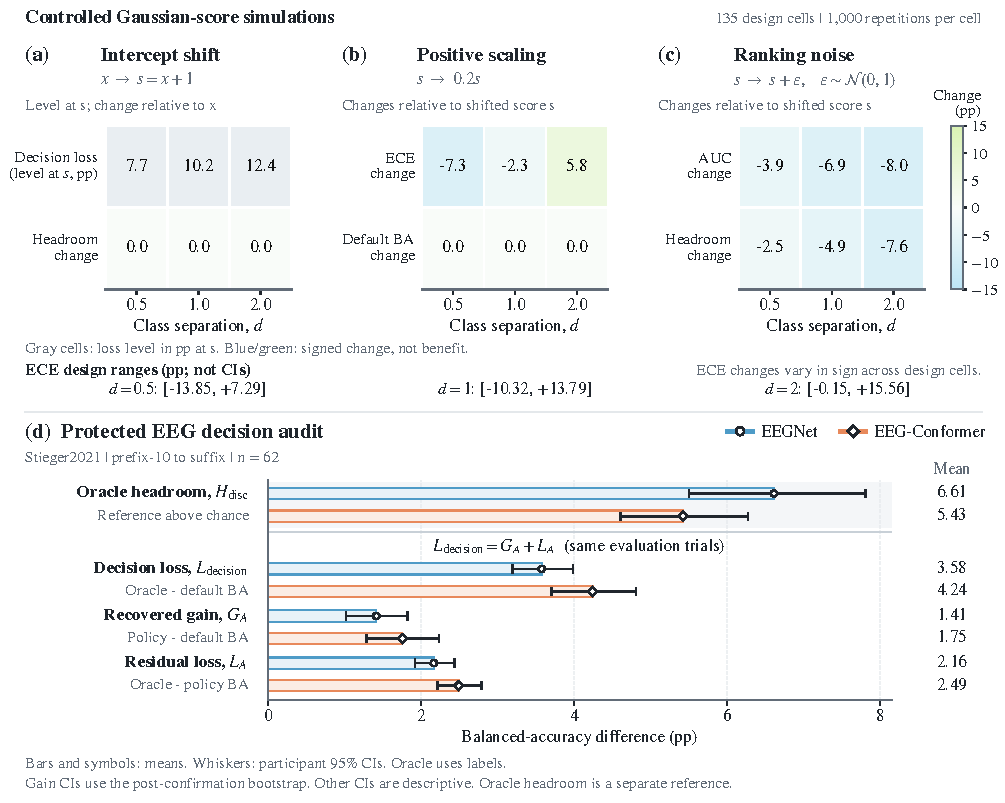
\includegraphics{figures/figure2_construct_protected_audit.pdf}
\caption{Known score interventions and the protected Stieger decomposition. (a)--(c) Each cell averages 45 design settings at the indicated class separation. The ECE ranges beneath the panels give the smallest and largest cell means at each separation. Intercept-shift loss is a level at the shifted score. Scaling and noise are changes relative to that score. (d) The 62 Stieger participants contribute model-averaged estimates on trials 11 onward. The whiskers give marginal 95\% participant intervals. The gain uses the post-confirmation participant bootstrap. The other component intervals are descriptive.}\label{fig:construct}
\end{figure*}

Figure~\ref{fig:construct}(a)--(c) distinguishes the changes in decisions, probability calibration and ranking. The intercept preserved empirical oracle headroom exactly but left 7.71--12.45 points of default decision loss on average across the three separation levels. Compression gave exactly the same default decisions in every repetition. Its mean ECE change was $-7.32$, $-2.31$ and $+5.85$ points as $d$ increased. Independent noise lowered both AUC and headroom at all three levels. The largest tested accounting residual was zero. A separate paired class-stratified normal interval targeted population BA loss between the \emph{known} Gaussian-optimal threshold and zero. Its lowest coverage across cells with $n\geq160$ was 92.8\%, above the 92\% gate and below nominal 95\%. This check concerns that interval and known threshold. EEG sampling uncertainty and fitted-oracle optimism require separate evidence.

A balanced prior also leaves the threshold unidentified. Consider equiprobable scores $-3,-2,\ldots,4$ and the following two monotone right-class probabilities, in percent, in score order. World A has $(1,1,49,49,60,60,80,100)$ and world B has $(0,40,55,55,60,60,65,65)$. Both have prior 0.5. Enumerating the nine threshold splits gives optimal BA of 0.75 for a threshold in $(0,1]$ in A and 0.65 in $(-2,-1]$ in B. The score marginal and prior available to the policy are identical. This construction limits what can be inferred from observed success of a median rule.

\subsection{Discovery and locked confirmation}
\begin{figure}[t]
\centering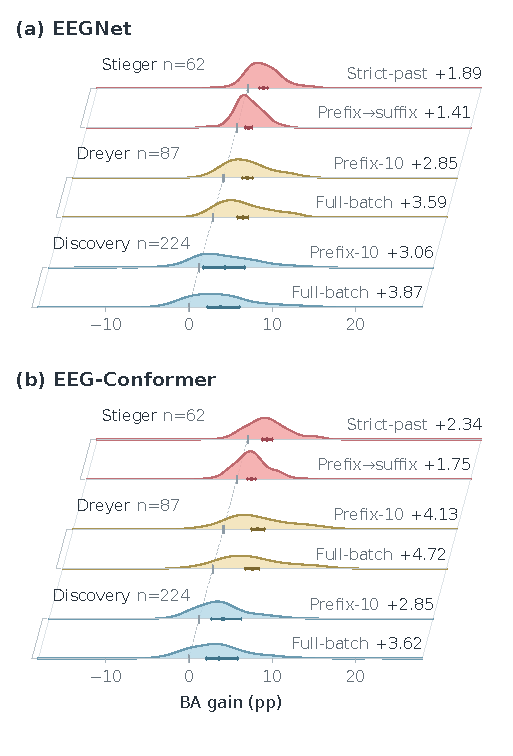
\includegraphics{figures/figure2_cross_cohort_forest.pdf}
\caption{Prior-quantile gain over the matched default decision. Dots show mean gains. Bars give 95\% bootstrap intervals from the discovery and Dreyer analyses and the post-confirmation participant bootstrap for Stieger. Ridges show Gaussian densities of participant gains on a shared scale with Scott bandwidths. Depth separates endpoints. Within a cohort the same people contribute to each row. Historical prefix and batch score the complete record. Stieger prefix and strict-past score trials 11 onward.}\label{fig:cohorts}
\end{figure}

In Fig.~\ref{fig:cohorts}, the discovery prefix-ten gains were 3.06 [0.50, 5.42] and 2.85 [1.43, 5.01] BA points for EEGNet and the Conformer, respectively. Full-batch gains were 3.87 [2.23, 6.08] and 3.62 [2.13, 5.85]. Discovery intervals resample datasets, protocols and participants hierarchically. Dreyer and Stieger intervals resample participants after source and seed averaging. After aggregation within participants, historical prefix ten gave a negative gain for 20.5\% of EEGNet and 19.2\% of Conformer participants in discovery. The fifth percentiles of gain were $-2.00$ and $-1.71$ points. The archived discovery tail non-degradation criterion failed. Discovery stores probabilities, some saturated, so converting them back to logits cannot recover the original score ordering at the extremes. Its decision results can be used at their recorded precision.

On Dreyer, prefix-ten gains were 2.85 [2.29, 3.45] and 4.13 [3.36, 4.91] points. Complete-batch gains were 3.59 [2.98, 4.24] and 4.72 [3.88, 5.56]. Default BA was 55.33\% for EEGNet and 51.66\% for the Conformer. Historical prefix ten retained 79.3\% and 87.3\%, respectively, of each model family's complete-batch gain. At the historical prefix endpoint, 11.5\% and 9.2\% of participants respectively lost accuracy. Both backbones met the secondary 75\% recovery criterion and the complete-batch magnitude and interval criteria. However, mean participant AUC was 0.620 and 0.585 against a required 0.60. Changing raw-BN to raw-GroupNorm gained 5.02 and 1.55 points against a two-point criterion. Only EEGNet met both of these primary gates. Worst-participant BA under complete-batch repair fell from 47.14\% to 47.03\% for EEGNet and from 49.81\% to 47.06\% for the Conformer. A lower minimum describes the cohort tail and need not refer to the same individual before and after repair.

\subsection{Protected external endpoint}
\begin{table}[t]
\caption{External cohort, 62 participants. Top rows give absolute percentages on the protected suffix for prefix ten. Bottom rows give prior-quantile gains in points versus the default on each rule's evaluation rows (Table~\ref{tab:contracts}). Brackets give marginal 95\% participant intervals. Gain intervals use the post-confirmation bootstrap.}\label{tab:primary}
\centering\small\setlength{\tabcolsep}{4pt}\begin{tabular}{@{}lrr@{}}\toprule
Protected measure (\%) & EEGNet & Conformer \\\midrule
Default BA & 53.04 [52.26, 53.90] & 51.18 [50.85, 51.55] \\
Quantile BA & 54.45 [53.38, 55.60] & 52.93 [52.19, 53.67] \\
Rank AUC & 57.02 [55.39, 58.75] & 54.95 [53.80, 56.11] \\
Oracle BA & 56.61 [55.50, 57.81] & 55.43 [54.60, 56.28] \\
\midrule Gain by access (pp) & EEGNet & Conformer \\\midrule
Fixed prefix 10 & 1.41 [1.01, 1.82] & 1.75 [1.28, 2.23] \\
Strict past & 1.89 [1.40, 2.39] & 2.34 [1.75, 2.95] \\
Session forward & 1.63 [1.14, 2.11] & 2.07 [1.50, 2.66] \\
Complete batch & 1.89 [1.40, 2.40] & 2.42 [1.84, 3.03] \\
\bottomrule\end{tabular}
\end{table}

The frozen external models produced 30 score streams over the same 69,628 distinct Stieger trials. The protected median sees ten unlabeled scores per participant and predicts on trials 11 onward. Table~\ref{tab:primary} pairs each gain with its default, its final accuracy and the BA attainable with suffix labels. Moving the threshold raised BA from 53.04\% to 54.45\% for EEGNet and from 51.18\% to 52.93\% for the Conformer. The participant-bootstrap intervals for gains of 1.41 and 1.75 points both exclude zero. Both point estimates fall short of the two-point magnitude criterion. The Conformer interval crosses two points, but its point estimate determines the branch. The protected conclusion remains \emph{mixed}.

AUC exceeds chance, yet even the fitted static oracle attains only 56.61\% and 55.43\% BA on average. Figure~\ref{fig:construct}(d) places these measurements on a common BA-difference scale. The estimated default decision loss is 3.58 and 4.24 points. After prefix fitting, 2.16 and 2.49 points remain between the policy and the label-informed static reference. The accounting relation holds before rounding. Separate marginal intervals for its terms need not add. This combination of working threshold repair and limited absolute discrimination constrains the practical interpretation.

\begin{table*}[!t]
\caption{Changing fitting budget and evaluation start. Historical moving-suffix columns show mean BA gains in points. The post-hoc common suffix includes marginal 95\% descriptive intervals, using the same 10,000 participant draws across budgets. Each pair lists EEGNet then Conformer.}\label{tab:common}
\centering\small\begin{tabular}{@{}lrrrrrr@{}}\toprule
$k$ & Fixed, Net & Fixed, Conf. & Past, Net & Past, Conf. & Common, EEGNet & Common, Conformer \\\midrule
5 & 1.22 & 1.70 & 1.88 & 2.34 & 1.19 [0.85, 1.54] & 1.67 [1.23, 2.12] \\
10 & 1.41 & 1.75 & 1.89 & 2.34 & 1.38 [0.98, 1.78] & 1.72 [1.24, 2.20] \\
20 & 1.51 & 1.90 & 1.88 & 2.34 & 1.50 [1.07, 1.92] & 1.87 [1.36, 2.39] \\
50 & 1.59 & 1.95 & 1.86 & 2.33 & 1.59 [1.13, 2.04] & 1.95 [1.42, 2.46] \\
\bottomrule\end{tabular}
\end{table*}

\subsection{Access windows and the cost of moving the test set}
Strict-past refitting yielded 1.89 and 2.34 points on the same trials 11 onward as the fixed-prefix rule (Table~\ref{tab:primary}). Both the amount of available past data and the opportunity to update change. A first-session fit is held fixed on subsequent sessions, so it tests transfer across acquisitions. The full-batch threshold reads future scores and evaluates early trials too. Under strict-past updating, 19 of 930 EEGNet and 28 of 930 Conformer participant--model rows exceeded their in-sample static oracle, producing a negative signed residual. No participant had a negative mean residual after model averaging. A larger cohort mean in one of these rows alone provides no chronological comparison of deployable policies.

In the historical $k$ sweep, fixed-prefix accuracy is evaluated on $k+1,\ldots,n$. Changing $k$ alters both the fit and the test set. In the corresponding strict-past sweep, increasing $k$ only postpones the evaluation start. The prediction for a shared trial still uses all its predecessors. To isolate fitting budget, the post-hoc analysis fixes the evaluation rows at $51,\ldots,n$ for $k=5,10,20,50$. It requires the same eligible participants and 15 models per backbone at every budget. Scores between the fit and trial 51 are unavailable to the fitted threshold. The common-window design was specified after the historical study and before this comparison was computed.

All 62 participants contributed the same 66,528 distinct suffix trials under every budget. From five to fifty available scores the mean gain changed from 1.19 to 1.59 points for EEGNet and from 1.67 to 1.95 for EEG-Conformer. These estimates describe budget sensitivity on a fixed sample. They do not select a deployment budget or revise the protected gate.

Table~\ref{tab:common} reports all four budgets, including those between the two extremes. For example, the protected $k=10$ and the common-window $k=10$ use identical fitted thresholds. Their different gains measure the effect of scoring different rows. Neither the moving-window sequence nor the marginal intervals constitute a paired test for an optimal $k$.

\subsection{Access-matched controls and their adverse outcomes}
A source-only Youden threshold gained 0.68 points [0.49, 0.89] for EEGNet and 0.84 [0.60, 1.09] for the Conformer on the protected suffix. Source intercept and source Platt moved the decision less, yielding mean gains between 0.16 and 0.30 points. Positive temperature left every zero-logit decision unchanged. For the paired cutoff comparison on the same Platt-v2 fit, changing the source cutoff from 0.5 to $\pi_s$ changed gain from 0.23 to 0.27 points for EEGNet and from 0.30 to 0.27 for the Conformer. Access to validation labels and the choice of utility both matter even before a target score is observed.

\begin{table}[t]
\caption{Protected suffix by policy. The last two columns count participants with negative gain and gain below $-2$ points, respectively, out of 62, after averaging over models. Source Platt is source-only. The remaining rules read the first ten target scores. EM and BBSE additionally use the fitted source map.}\label{tab:policies}
\centering\footnotesize\begin{tabular}{@{}lrrrr@{}}\toprule
Backbone & Policy & Gain [95\% CI] & $<0$ & $<-2$ \\\midrule
EEGNet & Source Platt & 0.23 [0.13, 0.32] & 20 & 0 \\
EEGNet & Prior quantile & 1.41 [1.01, 1.82] & 9 & 1 \\
EEGNet & Platt--EM & -2.48 [-3.12, -1.89] & 55 & 29 \\
EEGNet & Ridge BBSE & -2.33 [-2.92, -1.76] & 55 & 27 \\
Conformer & Source Platt & 0.30 [0.16, 0.46] & 19 & 0 \\
Conformer & Prior quantile & 1.75 [1.28, 2.23] & 11 & 1 \\
Conformer & Platt--EM & -1.00 [-1.29, -0.75] & 52 & 11 \\
Conformer & Ridge BBSE & -1.01 [-1.28, -0.76] & 53 & 11 \\
\bottomrule\end{tabular}
\end{table}

Table~\ref{tab:policies} shows the contrast within the protected target window. Both posterior-at-0.5 corrections reduced participant-averaged BA for most participants. Changing the Ridge BBSE shrinkage over the prespecified values retained negative mean gains. In particular, EEGNet's EM rule lost more than two points for 29 of 62 participants. The shared ten-score budget alone does not determine the direction of a change. Prior estimation, source calibration and the decision objective can all affect these results. The observed deficits cannot identify which assumption failed.

Target-signal methods can also change the score ranking. In historical paired comparisons against each corresponding frozen raw-BN checkpoint (224 participants), full-signal AdaBN gained 5.78 EEGNet and 4.30 Conformer points. Sequential TENT changed BA by $-4.86$ and $-0.65$ points, and T3A by $-1.12$ and $-0.97$~\cite{wang2021tent,iwasawa2021}. The official T-TIME port used a distinct matched baseline, its IEA-only component~\cite{li2024ttime}. Aggregating 2,688 paired participant-run differences within the 224 participants gave $-2.38$ BA points and $-4.58$ AUC points. A ranking change is possible in this block. These runs use historical target signals and their own matched baselines, which precludes a performance ordering with the Stieger score-only policies.

\section{Robustness and participant heterogeneity}\label{sec:heterogeneity}
\subsection{Source conditions and repeat seeds}
Checkpoint quality also varied before target access. On source-validation participants, checkpoint-mean BA ranged from 50.00\% to 78.36\% for EEGNet and 50.00\% to 72.82\% for the Conformer. Those participants contributed to checkpoint selection. The ranges provide context for the frozen conditions and cannot establish out-of-sample source performance.

Figure~\ref{fig:source_omission} holds the target cohort and prefix-ten policy fixed. At each spoke we omit one training condition from the summary of existing checkpoints. For each seed, we average gains over the four retained conditions within each participant, then over the same 62 Stieger2021 participants. All ten cross-seed omission means are positive. Positive leave-one-condition-out averages do not imply positive gains for every individual source condition. On the same 62 participants, the Conformer trained on BNCI2014-001 alone averaged $-0.323$ points across its three seeds. Two Conformer seed means fall just inside the zero ring. Omitting LODO gives $-0.08$ points at seed 17, and omitting Lee2019-MI gives $-0.04$ at seed 43.

\begin{figure}[t]
\centering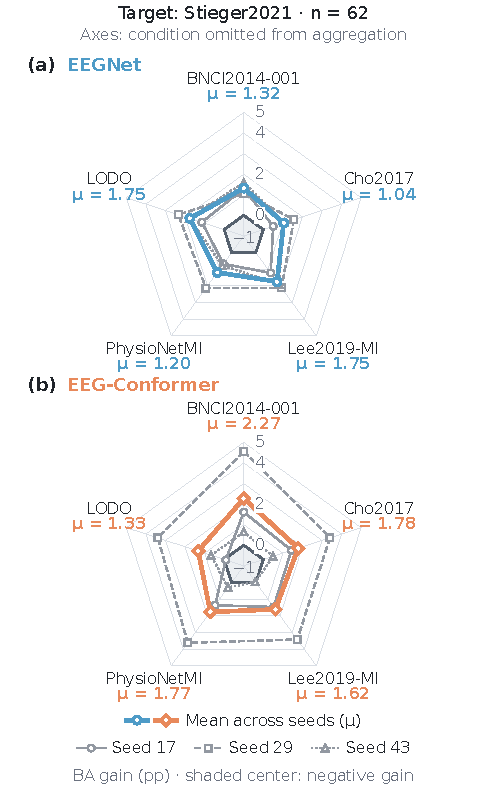
\includegraphics{figures/figure4_source_robustness_radar.pdf}
\caption{Training-source omissions on the protected Stieger suffix. Every spoke omits the named training condition from aggregation, with all checkpoints frozen. LODO denotes the multi-source condition. Gray contours describe seeds 17, 29 and 43. The colored contour and $\mu$ labels give their mean. Both panels use the same linear scale from $-1$ to $+5$ BA points. The bold zero ring encloses negative gains. Seed contours convey no confidence interval. Performance comparisons use spoke values and exclude polygon area.}\label{fig:source_omission}
\end{figure}

The participant bootstrap asks how the mean would vary with the participant sample at this fixed model grid. A second weighting first averages participants within each training condition and resamples the five condition means. The resulting gain intervals widen to [0.40, 2.42] points for EEGNet and [0.60, 2.75] for the Conformer. Dataset-balanced weighting equals participant weighting on a single external dataset. None of these intervals measures variation across newly trained backbones or unobserved acquisition sites.

\begin{table}[t]
\caption{Between-seed Spearman correlations of participant gain on the protected suffix. For each backbone and seed, gains are averaged over all five training conditions before ranking the same 62 participants.}\label{tab:robust}
\centering\small\begin{tabular}{@{}lrr@{}}\toprule
Seed pair & EEGNet & Conformer \\\midrule
17 vs. 29 & 0.70 & 0.77 \\
17 vs. 43 & 0.57 & 0.31 \\
29 vs. 43 & 0.82 & 0.44 \\
\bottomrule\end{tabular}
\end{table}

Table~\ref{tab:robust} shows how consistently the seeds rank participants by gain. Agreement varies especially for the Conformer, from 0.31 to 0.77. Participants, training conditions and seeds recur across the omission contrasts.

\subsection{Oracle transfer across sessions}
\begin{figure}[t]
\centering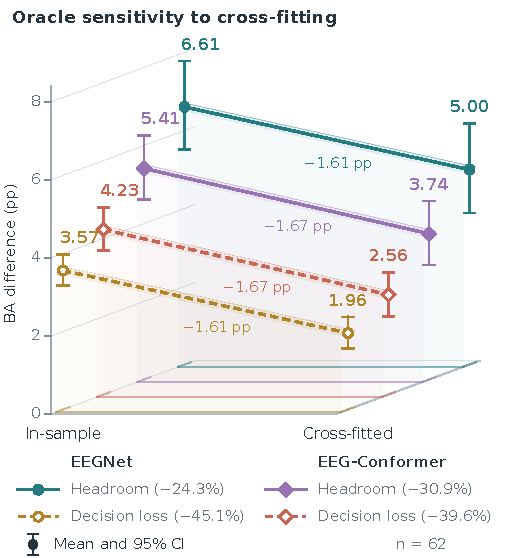
\includegraphics{figures/figure6_oracle_sensitivity.pdf}
\caption{Oracle sensitivity on complete eligible Stieger sessions. The in-sample threshold uses all eligible trials of a participant. Cross-fitting predicts each held session using labels from the other sessions. Decisions from the held sessions are pooled for BA on the same complete records. Points and whiskers are means and marginal 95\% participant intervals ($n=62$). Connecting segments show point changes. Relative reductions use the corresponding in-sample mean.}\label{fig:oracle}
\end{figure}

The leave-one-session-out replay evaluated 17,760 model--participant--session folds across the 30 models. Each participant contributed at least two eligible sessions and no model-session fold was excluded. Moving the threshold fit off the held session reduced EEGNet decision loss from 3.57 to 1.96 points and Conformer loss from 4.23 to 2.56 (Fig.~\ref{fig:oracle}). The corresponding held-session 95\% intervals were [1.56, 2.38] and [2.00, 3.13] points. Mean headroom fell from 6.61 to 5.00 [3.89, 6.19] points and from 5.41 to 3.74 [2.94, 4.58]. These estimates provide a reference for transferring a threshold across sessions, including sessions later in acquisition order. Subtracting the protected prefix gain would mix different sets of trials.

\subsection{Counting at a fixed model}
\begin{figure}[t]
\centering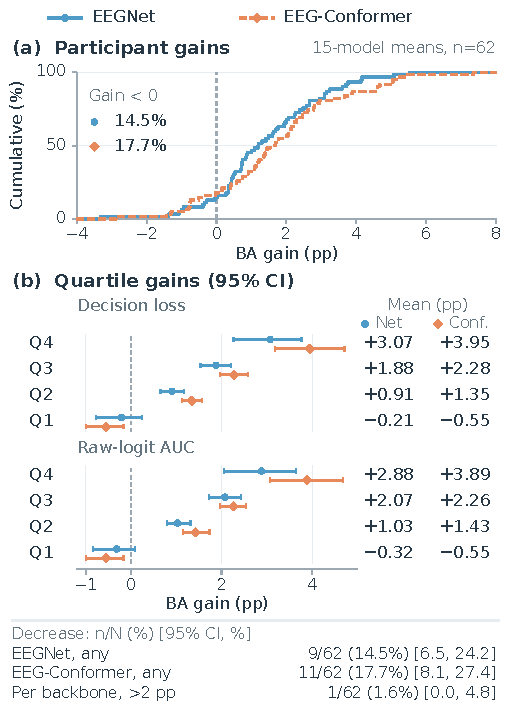
\includegraphics{figures/figure7_participant_degradation.pdf}
\caption{Participant gains on the protected suffix after averaging 15 source-condition/seed configurations within each participant and backbone. (a) Empirical cumulative distributions and fractions below zero. The footer gives the resulting participant counts and rates for each backbone. (b) Mean gains and 95\% participant intervals by within-backbone decision-loss or AUC quartile. Quartile sizes are 16, 15, 15 and 16. Intervals condition on the original membership. The same participant can occupy different quartiles across stratifiers and backbones.}\label{fig:strata}
\end{figure}

The median participant gain after averaging models was 1.19 points for EEGNet and 1.62 for the Conformer. Nine and eleven of the 62 participants, respectively, had negative averages. Each backbone had one participant with a decrease exceeding two points, or 1.6\%. The original percentile interval for this rare count is 0.0--4.8\%. A Wilson sensitivity gives 0.3--8.6\%, conditional on the observed classifications. With one event, neither interval gives a stable upper bound on the risk to a future individual.

For a fixed checkpoint, we instead counted participants with gain strictly below $-2$ BA points before aggregating across models. Using the same 62 participants for every checkpoint, EEGNet's 15 counts ranged from 1/62 to 14/62, compared with 1/62 after averaging. The 15 Conformer counts ranged from 0/62 to 17/62, also compared with 1/62 after averaging. No model was selected using these counts. They describe retrospective heterogeneity conditional on model identity.

Figure~\ref{fig:strata} locates the negative tail after model averaging. Each curve contains one gain per participant. In the lowest AUC quartile, mean gains were $-0.32$ and $-0.55$ points, with 8/16 and 11/16 participants below zero. In the highest AUC quartile the means rose to 2.88 and 3.89 points. The decision-loss quartiles show a related gradient. Gain and decision loss share the default BA term, and the in-sample oracle constrains recoverable gain for a static policy. These strata use outcomes from the evaluated suffix and cannot select participants in advance. A positive cohort mean, seed-to-seed agreement and the degradation count for a named checkpoint convey distinct evidence about transfer.

\section{Interpretation and reproducibility}\label{sec:limits}
\subsection{What an access-conditioned benchmark can establish}
The same ten-score threshold defines different experiments depending on whether its warm-up is scored. A common evaluation mask addresses that ambiguity directly. The same set of participant--model outcomes also gives different counts according to whether thresholding for a large decrease precedes or follows model averaging. Retaining participant, model and session keys until the final aggregation makes these choices reviewable. This matters when a benchmark serves both retrospective comparison and a decision about one deployed checkpoint.

Adaptive decision boundaries have a precedent in motor-imagery BCI. PMean updates an LDA bias from a running pooled feature mean under a fixed separation model, and its feedback experiment supplied feedback using the PMean rule itself~\cite{vidaurre2011}. The present median rule uses recorded deep-model scores and leaves all feature weights fixed. Here the participant cannot respond to a changed decision. Likewise, methods such as Average Thresholded Confidence seek to predict target accuracy in the absence of target labels~\cite{garg2022atc}. ACDD uses labels retrospectively for evaluation and diagnostic oracles. A fitted rule can improve without providing an unlabeled estimator of its own performance.

The scope is six public cohorts of cued binary left/right imagery, two backbones, one common sensor montage and a declared balanced prior. A different prevalence, a different cost for errors, class abstention or a new montage can change which comparison is relevant. Source validation was reused for checkpoint selection and calibration. Decreases in BA describe classification outcomes. They do not measure an injury or adverse clinical event. Prospective feedback, asynchronous or multiclass control, future users, and other time-series domains require separate experiments.

\subsection{Artifact, provenance and reproducibility}
The local artifact identifies the 30 paired-logit target files, labeled source-validation inputs and checkpoint hashes. With recorded scores, its first group of calculations reconstructs the protected decisions, common-suffix decisions and cross-fitted references. A source-only refit of Platt-v2 reproduces the persisted parameter values at full precision. Loading those verified snapshots regenerates the decision hashes, 59,520 candidate participant--model--policy rows and 1,860 paired utility rows. The source-only, EM and BBSE controls in Table~\ref{tab:policies} use this version. The protected quantile uses no Platt parameters.

The historical Platt coefficients were unavailable. Against archived BA, a legacy refit changed 116 of 14,880 protected participant--model--policy rows (62 source Platt and 54 EM, one EEGNet checkpoint). The largest absolute difference was 2.98 points. Separately, Platt-v2 changed 1,516 of 59,520 rows across four windows at tolerance $10^{-12}$, with a maximum of 6.47 points. In Table~\ref{tab:policies}, its protected EEGNet EM mean moved from $-2.512$ to $-2.484$ points and its count below $-2$ fell from 32 to 29. For Conformer source Platt, 19 participants had negative mean gain, compared with 22 historically. All eight gain intervals retained their direction. The median policy, its fixed-model counts and the raw-logit oracles use no fitted Platt map.

The archived discovery input begins at participant metrics. Dreyer starts from trial predictions, and the synthetic study regenerates scores from its design. Software, checkpoint locations and official acquisition paths are identified for the EEG-to-logit path. Raw-signal replay and end-to-end temporal invariance were not run. The historical registry for Fig.~\ref{fig:cohorts} names one CSV for all four Stieger rows but carries the digest of the earlier confirmation JSON. Both files are available. Their four means agree, while all four bootstrap intervals differ. The confirmation analysis resampled participant means and used order-statistic limits. Its protected gain intervals were [1.02, 1.81] points for EEGNet and [1.28, 2.25] for the Conformer. The plotted intervals use interpolated percentiles from the later participant bootstrap after averaging seeds and source conditions. Replaying the two score rules and that bootstrap reproduced all four plotted triples. The candidate manifest pairs each file with its own digest and records the bootstrap used for the plotted intervals. The author archive contains the verified frozen inputs. The reviewer package lists each restricted input by digest. Its distribution route and public artifact URL await author approval.

\subsection{Ethics}
The study reuses public de-identified recordings and involved no new recruitment. Original sources document oversight and consent for Cho2017, Lee2019-MI, Dreyer2023 and Stieger2021. The records reviewed for BNCI2014-001 and PhysioNetMI did not establish those details. The authors' institutional determination for secondary use awaits confirmation.

\section*{Acknowledgments and AI-generated content}
In earlier revisions, OpenAI Codex assisted with drafting and revising Sections I--VI, literature retrieval, code inspection and scripting for the frozen-score replay, the common-suffix calculation and table construction. It also assisted with numerical and layout checks and artifact documentation. The workflow and five result figures reuse the earlier manuscript's artwork. Edits to the workflow and participant figure clarify the score interface and the aggregation unit. In the preceding submission-preparation pass, its review of the scientific prose was limited to grammar. For this edition, Codex helped clarify trial eligibility and implement and test the reproduction package. Author review of the interpretation and final disclosure is pending.

\bibliographystyle{IEEEtran}
\bibliography{references}
\end{document}
